\section{Results} \label{Results}
The framework detailed before is used to generate the results presented in this section. First, the case study is explained as well as the format used to present the results. Then an interpretation of the results is proposed.

\subsection{Case study}
At this point, it is possible to study a wide variety of flight configuration and situations. To keep the study consice we will limit our analysis to the situation of engine failures at take off with landing gear retracted as described by CS25.121, CS25.147 and CS12.149 \cite{CS25}. These certification rules set the requirements on climb angle, directional control and $V_{MC}$ in case of one or multiple engine failures. Although this manner bounds the study to only one flight phase, a good insight is given on the tool efficiency to compare aircraft configuration and potential of differential thrust.

The certification rules indicate different flight conditions for twin engine and aircraft with more than four engines. The main differences are resumed in table~\ref{tab:DiffTwinMulti}. %CS25.121 states the following flight conditions:
\begin{table}[hbt]
	\caption{\label{tab:DiffTwinMulti} Certification requirements for twin-engines and more than four engines \cite{CS25}} 
	\centering
	\begin{tabular}{l|l|c}
		Parameters & Twin engine & More than four engines\\
		\hline
		Gradient of climb, critical engine inoperative & $\leq 2.4\%$ & $\leq 3.0\%$\\
		Heading change of $15\degree$ at 1.3$V_{SR_1}$& One engine inoperative & Two critical engines inoperative\\
		$V_{MC} < 1.13 V_{SR}$ & One engine inoperative & One critical engine inoperative \\
	\end{tabular}
\end{table}

It is of interest to investigate the most defavorable situation for differential thrust which is clearly at a $3\%$ climb angle and two or more critical engines inoperative. 

For aircraft with more than four engines, the certification specifies that sufficient control must remain possible with the two critical engines inoperative at $1.3V_{SR}$ to perform heading changes. While $V_{MC}$ has to be demonstrated with two engines inoperative only at landing where fuel shortage is expected. This is not as constraining as for the take off where a much higher power is needed. A carefully designed architecture would normally avoid the suddent stop of engines located one next to another as in the case of Ampere \cite{Ampere_concept}. Other risks however might damage closely located engines such as bird collision or rupture of a propeller.

For these reasons it has been decided to render at least three engines inoperative, representing one fourth of the total power. Thus the total number of engines for the ATR72 with DEP is fixed to twelve.

A total of four configurations are studied to capture the overall changes that differential thrust and VT reduction bring to the aircraft. These configurations are resumed in table~\ref{tab:ConfigurationStudied}. It must be stressed that velocities are calculated from publicly available data and thus are only indicative \cite{ATRspeed}.


\begin{table}[hbt]
	\caption{\label{tab:ConfigurationStudied} Aircraft Configurations}
	\centering
	\begin{tabular}{l|c|c|M{3cm}|M{3cm}}
		Configuration & Original & DEP 1 & DEP 2 & DEP 3\\
		\hline
		Description & Original ATR72 & DEP ATR72 & DEP ATR72 Differential Thrust & DEP ATR72 Differential Thrust and small VT\\
		\hline
		Engines & 2 & 12 & 12 & 12\\
		Inoperative engines & 1 & 3 & 3 & 3\\
		VT area & $S_{v_0}$ & $S_{v_0}$ & $S_{v_0}$ & $0.7 S_{v_0}$\\
		Rudder allowed & Yes & Yes & No & No\\
		Gradient of climb & $3.0\%$ &$3.0\%$ & $3.0\%$ & $3.0\%$\\
		Turn rate, $\Omega$ (rad/s)& 0 & 0& 0&0\\
		Propeller & \multicolumn{4}{c}{Feathered, no drag assumed}\\
		\hline
		\multicolumn{5}{c}{Additional parameters} \\
		\hline
		$V_{\textrm{app}}$=$1.13V_{\textrm{app}}$ (m/s)& \multicolumn{4}{c}{56}\\
		$V_{\textrm{sr}}$ (m/s)& \multicolumn{4}{c}{50.5}\\
		$1.3V_{\textrm{sr}}$ (m/s)& \multicolumn{4}{c}{65}\\
		VT stall limit & \multicolumn{4}{c}{$\beta=15\degree$}\\
		\hline
		\multicolumn{5}{c}{Flight parameters for throttle repartition and rudder deflection}\\
		\hline
		$\beta$ & \multicolumn{4}{c}{$0\degree$}\\
		V(m/s) & \multicolumn{4}{c}{60}\\
	\end{tabular}
\end{table}

The flight conditions represent a rectilinear climb at constant velocity. The same climb angle is imposed for all configuration to allow comparison in an identical flight situation.
For each configuration an equilibrium map is built by swapping side slip angle and flight velocity. Along the flight envelop comes the rudder deflection and throttle repartition of a single equilibrium point. Side slip angle and velocity for this point is shown in table~\ref{tab:ConfigurationStudied}

%\begin{itemize}
%\item Climb gradient with one engine inoperative may not be less than 2.4\% for twin engines
%\item Climb gradient with one engine inoperative may not be less than 3\% for aircraft with four engines or more.
%\end{itemize}
\clearpage
\subsection{Flight envelop map}
\subsubsection{Map Interpretation}\label{MapInterpretation}
The flight envelops along with the accompaning throttle repartition and rudder deflection are shown in Fig~\ref{MapOrignialTwin+DEP} to Fig~\ref{fig:DEPfin07_15enginesMap+Defl}. For each equilibrium map, a point indicates an equilibrium. If this equilibrium is on the edge of the stability map a line shows the limiting parameter. It is either the $5\degree$ limitation in roll, stall or rudder saturation.
For distributed propulsion, engine saturation is indicated with different markers. A rectangular marker signifies that one engine is saturated, up-triangle two engines, down triangle three engines, left triangle four engines and finally right triangle five engines.
Additionally, the complete zone after $\|\beta\|\geq 15\degree$ is faded, signifying that any equilibrium is valid under the condition that the VT did not yet experienced stall.

\subsubsection{ATR72 twin engine and Distributed propulsion}

The baseline ATR72 is presented in Fig~\ref{fig:originalfin1_3engine} and the trim inputs in Fig~\ref{fig:Defloriginalfin1_3engine}.
The climb gradient is slightly unfavorable for this configuration nevertheless, one can observe the compliance with the controlability requirement at low velocity and the $15\degree$ margin at $1.3V_{SR}$. The limiting parameters for the flight envelop are the roll angle limitation for negative side slipe, rudder deflection for positive side slipe. The map is not symmetrical as expected for the case of engine failure.

\begin{figure}[hbt]
	\centering
	\begin{subfigure}{0.49\textwidth}
		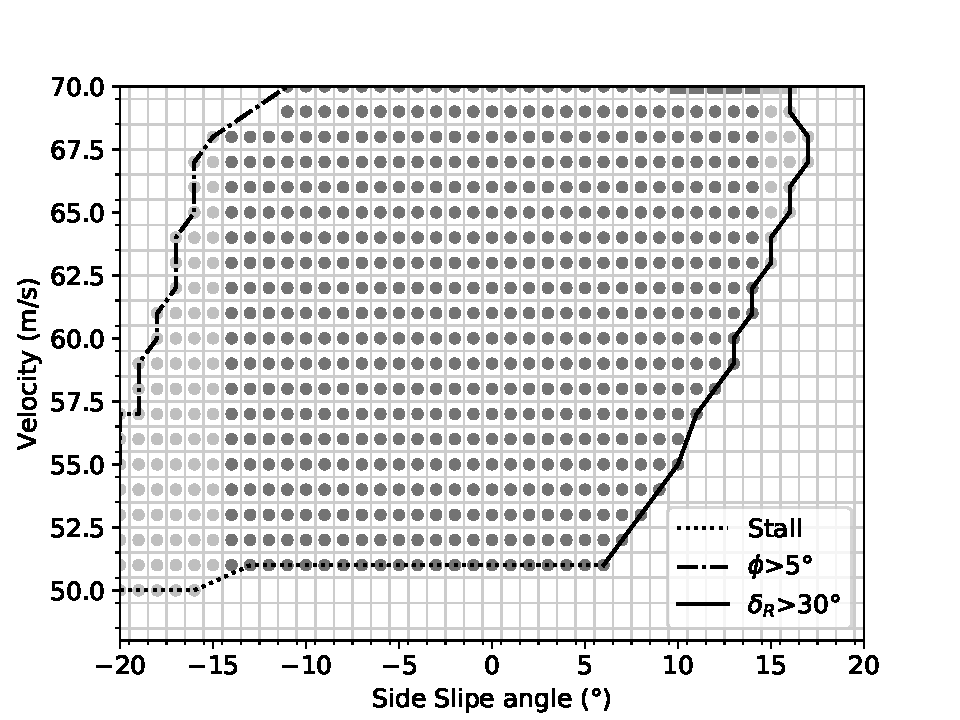
\includegraphics[width=0.95\textwidth]{originalMapBetaVelfin1Eng3RudFalse}
		\caption{Original ATR72, flight envelop.}
		\label{fig:originalfin1_3engine}
	\end{subfigure}
	\begin{subfigure}{0.49\textwidth}
		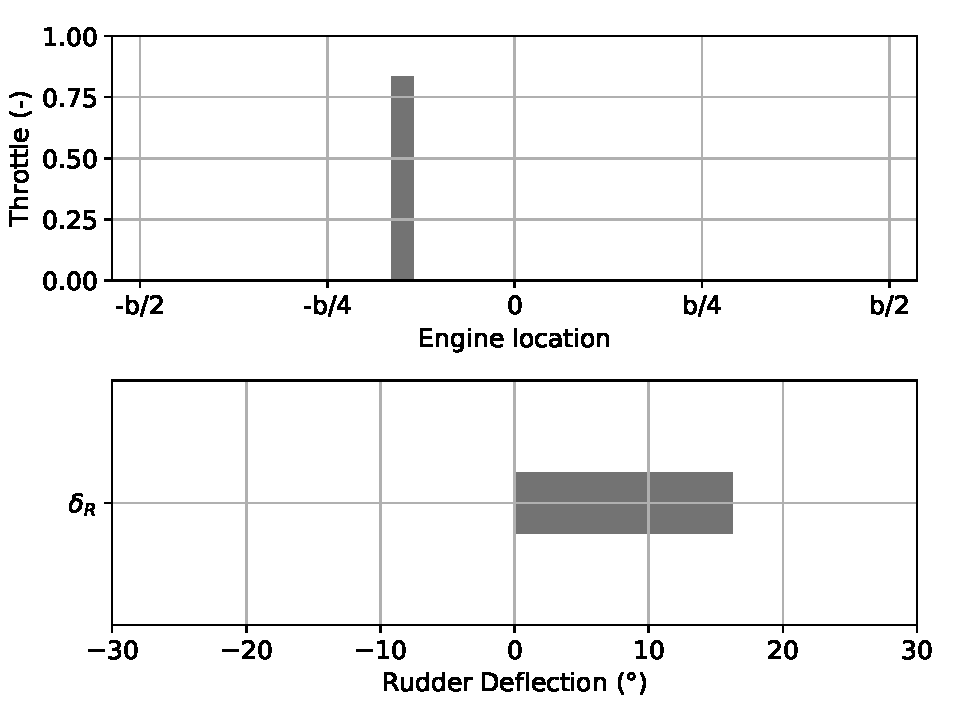
\includegraphics[width=0.95\textwidth]{Defloriginalfin1Eng3RudFalse}
		\caption{Original ATR72, throttle level and rudder deflection.}
		\label{fig:Defloriginalfin1_3engine}
	\end{subfigure}
	\caption{Map of equilibrium points of the Original configuration and throttle level and rudder deflection for trim at V=60m/s, $\beta=0$} \label{MapOrignialTwin+DEP}
\end{figure}

Fig~\ref{fig:originalfin1_15engine} and Fig~\ref{fig:Defloriginalfin1_15engine} show the same airplane equipped with a distributed propulsion however not using differential thrust as shown in Fig~\ref{fig:Defloriginalfin1_15engine}. Despite the fact that the power loss is only one fourth of the total power, rudder deflection remains similar to the previous case and the equilibrium map is only increased by a few degres to the right.

This can be reasonnably explained by the fact that the outter most engines on the left wing, despite representing only one fourth of the power, have a high level arm thus creating an important yaw moment. At this stage, designing an aircraft with Distributed Propulsion would not bring substantial reduction on the VT surface area since it remains the primary control effector for yaw. This changes once Differential Propulsion is activated.

\begin{figure}
	\begin{subfigure}{0.49\textwidth}
		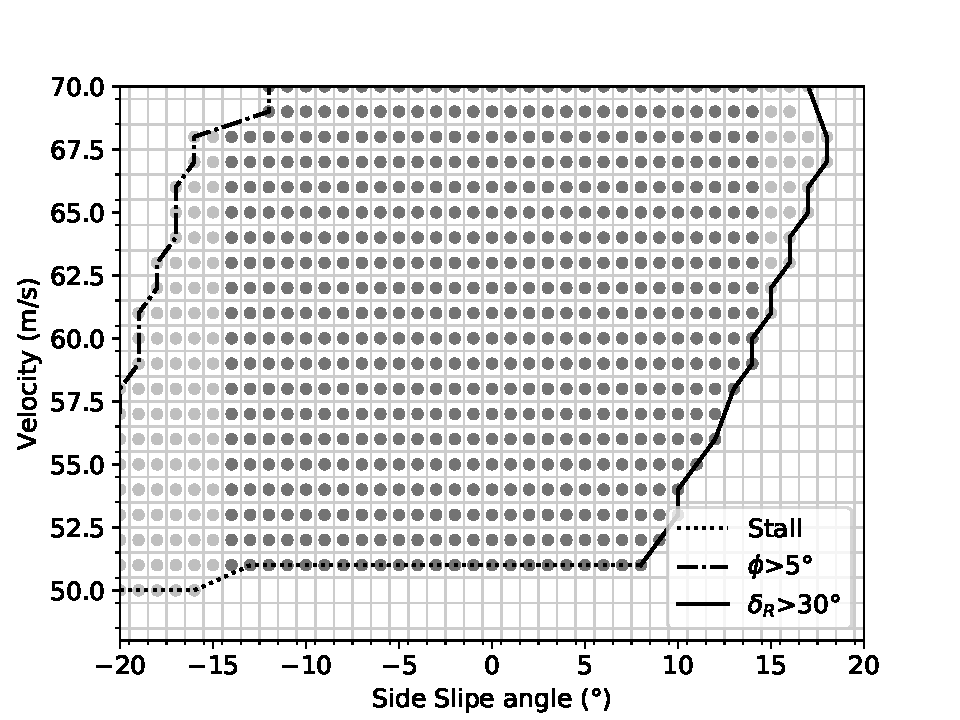
\includegraphics[width=0.95\textwidth]{originalMapBetaVelfin1Eng15RudFalse}
		\caption{DEP 1 flight envelop.}
		\label{fig:originalfin1_15engine}
	\end{subfigure}
	\begin{subfigure}{0.49\textwidth}
		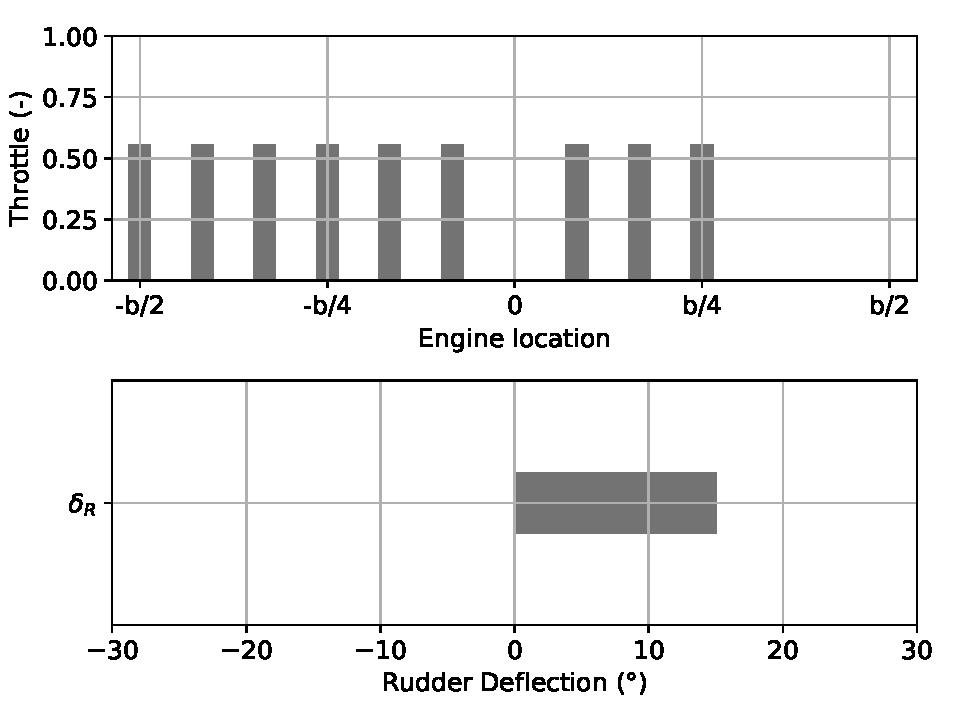
\includegraphics[width=0.95\textwidth]{Defloriginalfin1Eng15RudFalse}
		\caption{DEP 1, throttle level and rudder deflection.}
		\label{fig:Defloriginalfin1_15engine}
	\end{subfigure}
	\caption{Map of equilibrium points of the configuration DEP 1 and throttle level and rudder deflection for trim at V=60m/s, $\beta=0$} \label{DeflOrignialeNoDiffThrust}
\end{figure}

\subsubsection{ATR72 using differential thrust and small VT}
Fig~\ref{fig:DEPoriginalfin1_15engine} and Fig~\ref{fig:DeflDEPoriginalfin1_15Eng} respectively show the equilibrium map and the trim inputs for an ATR72 with distributed propulsion and differential thrust activated.

It is important to remember that to segregate the possible increase of control provided by the differential thrust, the rudder isn't activated for the remaing configurations as it is shown in Fig~\ref{fig:DeflDEPoriginalfin1_15Eng}. Continuing on the same figure, the thrust repartition found by the optimizer is linear except for the saturated engine(s) as it is the case here.

The equilibrium map shows one main characteristic intrinct to differential thrust: control power decreases with increasing velocity.

In consequence, since the flight enveloped is increased at low velocity with respect to Fig~\ref{fig:originalfin1_3engine} and Fig~\ref{fig:originalfin1_15engine}, it can be stated that differential thrust is able to maintain lateral control at low velocity. However at $1.3V_{SR}$ the control margin is too low.

\begin{figure}[hbt]
		\centering
		\begin{subfigure}{0.49\textwidth}
			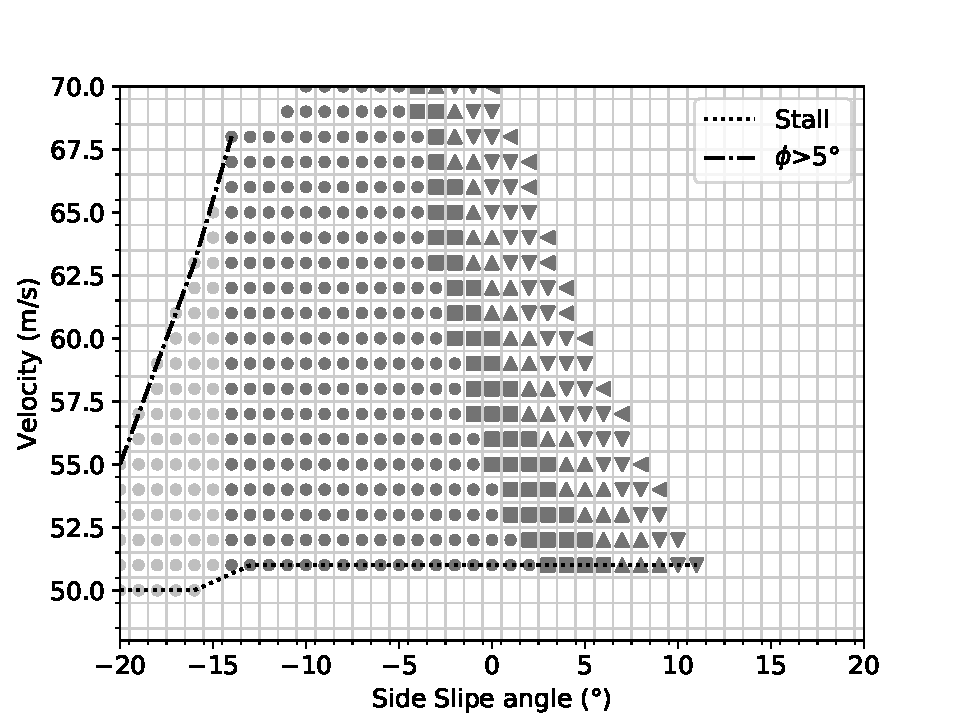
\includegraphics[width=0.95\textwidth]{DEPoriginalMapBetaVelfin1Eng15RudTrue}
			\caption{DEP 2, flight envelop.}
			\label{fig:DEPoriginalfin1_15engine}
		\end{subfigure}
		\begin{subfigure}{0.49\textwidth}
			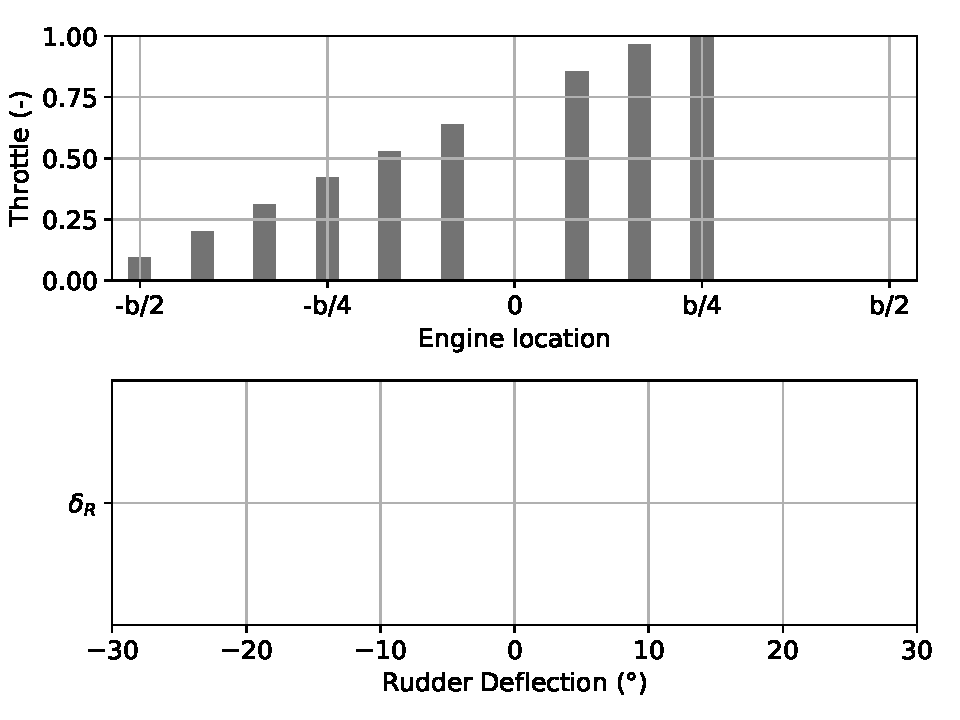
\includegraphics[width=0.95\textwidth]{DeflDEPoriginalfin1Eng15RudTrue}
			\caption{DEP 2, throttle level and Rudder deflection at 60m/s and $\beta=0\degree$.}
			\label{fig:DeflDEPoriginalfin1_15Eng}
		\end{subfigure}
		\caption{Configuration DEP 2 using only Differential Thrust. Rectangle indicate an equilibrium with one engine at saturation (full throttle), for map interpretation see paragraph \ref{MapInterpretation}}\label{DEPfin1_15engMap+Defl}
\end{figure}

The main reason why the flight envelop is reduced at high velocity is because the VT is generating a restoring moment as soon as side slip appears. To increase the flight envelop, one simply has to reduced the VT, which is performed in Fig~\ref{fig:DEPoriginalfin07_15engine} and Fig~\ref{fig:DeflDEPoriginalfin07_15Eng}. Here the VT surface area is reduced by $30\%$, the aircraft remains positively damped, that is $C_{n_\beta}>0$, however the equilibrium map improves vastly. The directional control margin at $1.3V_{SR}$ is now compliant with the certification despite the fact that a higher number of engines are being used at full throttle to maintain equilibrium.


\begin{figure}[hbt!]
	\centering
	\begin{subfigure}{0.49\textwidth}
		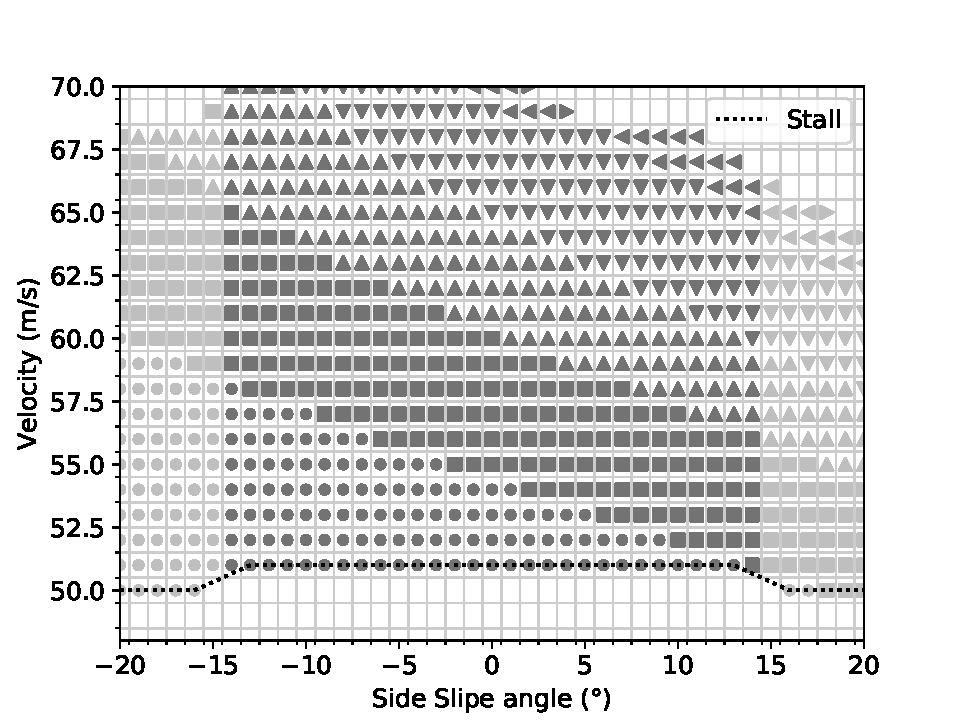
\includegraphics[width=0.95\textwidth]{DEPoriginalMapBetaVelfin07Eng15RudTrue}
		\caption{DEP 3, flight envelop}
		\label{fig:DEPoriginalfin07_15engine}
	\end{subfigure}
	\begin{subfigure}{0.49\textwidth}
		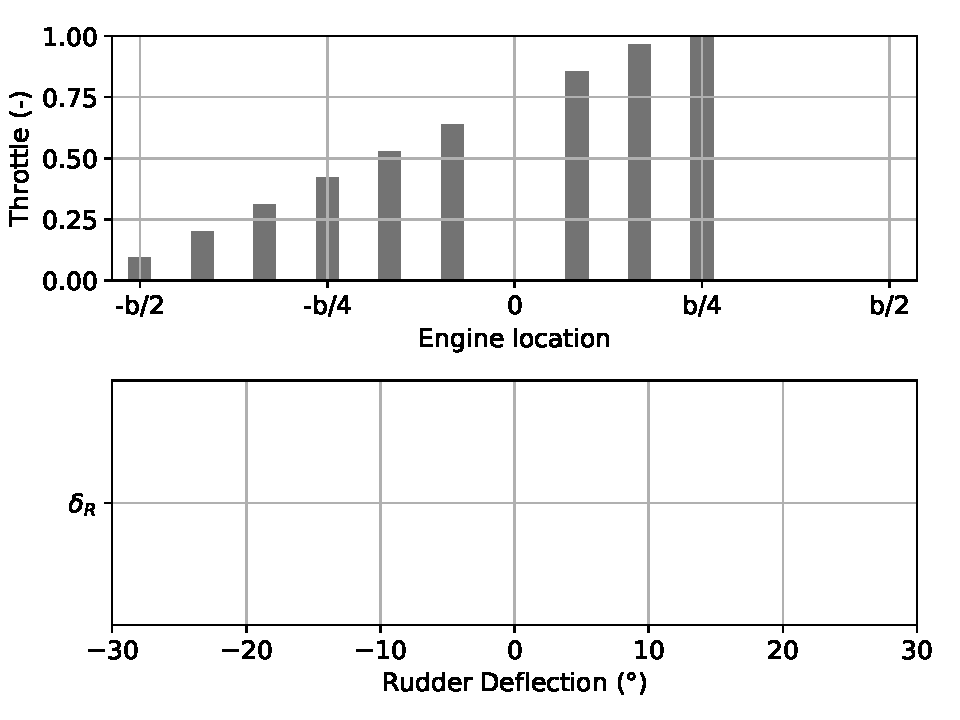
\includegraphics[width=0.95\textwidth]{DeflDEPoriginalfin07Eng15RudTrue}
		\caption{DEP 3, throttle level and rudder deflection at 60m/s and $\beta=0\degree$}
		\label{fig:DeflDEPoriginalfin07_15Eng}
	\end{subfigure}
	\caption{DEP 3, with $S_v=0.7S_{v_0}$. Rectangle indicates an equilibrium with one engine at saturation (full throttle), for map interpretation see paragraph \ref{MapInterpretation}}\label{fig:DEPfin07_15enginesMap+Defl}
\end{figure}

\subsubsection{Interpretation and limits of the results}
So far the following observation were made:
\begin{itemize}
	\item Equipping an ATR72 with distributed propulsion but not differential thrust would not guarranty a reduction of VT surface area due to the important level arm of engines located at the wing tip.
	\item Differential thrust alone would be sufficient to maintain full control of the aircraft at low velocity due to the high control effectiveness.
	\item The VT actually has to be reduced to be able to exploit the full potential of differential thrust.
\end{itemize}
\vspace{0.25cm}
Limitations can be anticipated if one extrapolates these results. The reduction of VT surface area could be further increased but then stability at high velocity, when differential thrust loses its control effectiveness would be badly degraded. This is observable as each aircraft employing differential thrust see their equilibrium map reducing with increasing velocity. Nevertheless this shows that employing differential thrust brings a new paradigm for the design of the VT by changing the design case.

The study is limited to the precision of the thrust model employed as well as the important assumption that no interaction takes place between propeller and wing. Models taking these effects into account can now be added to the framework.
The framework itself suffers from the underconstrained system of equations mostly when differential thrust and rudder are allowed together. It seems that the objective function doesn't induce enough constraints on the repartition of the yaw moment. The definition of an explicit allocation function could further increase the capability of the framework to predict trim points with differential thrust. Additionally, this study is limited by the aerodynamic models that consider non linear effects only with VT geometry and linear effects otherwise. That is no consideration of stall, efficiency decrease with rudder deflection or masking of VT by the fuselage.

As future work, implementation of interaction models and more precise thrust model has to be performed along with a better formulation for yawing moment distribution. In parallel of such development, the framework allows to study the dynamic behaviour of such configurations with or without stability augmentation system. It is also necessary to assess the variation of stability gains observed with the configuration i.d. the total number of engines, the ratio of inoperational engines as well as the total on board power. These will be part of future research in an effort to integrate this work in an multidisciplinary optimisation process for preliminary sizing.


%----- Study Case -----
%One original ATR72 at take off without failed engine next to the same ATR72 at Take off with SEF:
%	Shows that Vmc is found for take off,
%	Show that control is maintained at 1.3Vsr (=15° yaw toward inoperative engine)
%	shows that no equilibrium exists,
%	eventually show the degradation of equilibrium with reduced VT
%	Show the engine saturation at high speed

%Show the same ATR with distributed propulsion:
%	Show input histogramme with and without rudder
%	Show map without rudder and with small rudder
%	Show map with small fin and rudder
%
%At take off means :
%	3% slope for more than 4 engine condition, 
%	2.4 % for twin engine with landing gear retracted (CS.25.121)
%	Not necessarly full power but explore by going higher (in speed mostly)
%	0 altitude
%Maybe replace velocity scale by Vsr, 1.3Vsr etc... as defined by CS

% ATR at 21.5T Vapp=56m/s if it is 1.13Vsr then Vsr=49.55m/s, 1.3Vsr=64.4m/s
% Eventually look at the 20° turns requirement from the certif

%
%Determine 1.3V_{sr} for CS25.147 stating 15° yaw in the direction of the inoperative engine.
%STATE MINIMUM DRAG and 